\documentclass[a4paper]{article}

\usepackage[fontset=fandol]{ctex}
\usepackage{amsmath, amssymb}
\usepackage{graphicx}
\usepackage[margin=2.5cm]{geometry}
\usepackage[most]{tcolorbox}
\usepackage{etoolbox}
\usepackage{listings}
\usepackage{hyperref}
\usepackage{booktabs}
\usepackage{subcaption}
\usepackage{float}
\usepackage{tikz}
\IfFileExists{pgfplots.sty}{
    \usepackage{pgfplots}
    \pgfplotsset{compat=1.18}
}{}

\newtcolorbox{knowledgebox}[1]{
    enhanced, colback=blue!5!white, colframe=blue!75!black, colbacktitle=blue!75!black,
    coltitle=white, fonttitle=\bfseries, title=#1, attach boxed title to top left={yshift=-2mm, xshift=2mm},
    boxrule=1pt, sharp corners
}

\newtcolorbox{importantbox}[1]{
    enhanced, colback=yellow!10!white, colframe=yellow!80!black, colbacktitle=yellow!80!black,
    coltitle=black, fonttitle=\bfseries, title=#1, sharp corners
}

\newtcolorbox{warningbox}[1]{
    enhanced, colback=red!5!white, colframe=red!75!black, colbacktitle=red!75!black,
    coltitle=white, fonttitle=\bfseries, title=#1, sharp corners
}

\lstset{
    language=Python,
    basicstyle=\ttfamily\small,
    keywordstyle=\color{blue},
    stringstyle=\color{red!60!black},
    commentstyle=\color{green!60!black},
    breaklines=true,
    frame=single,
    numbers=left,
    numberstyle=\tiny\color{gray},
    captionpos=b,
    extendedchars=false
}

\newcommand{\notetitle}{CME 295 课程笔记：Lecture 1 Transformer}
\newcommand{\noteauthors}{Codex}
\newcommand{\notedate}{2026-04-13}
\newcommand{\videochannel}{Stanford Online}
\newcommand{\videopublishdate}{2025-10-17}
\newcommand{\videoduration}{1:41:59}
\newcommand{\videourl}{https://www.youtube.com/watch?v=Ub3GoFaUcds}
\newcommand{\videocoverpath}{cover.jpg}

\begin{document}

\begin{titlepage}
\centering
{\Large 课程笔记\par}
\vspace{1.2cm}
{\huge\bfseries \notetitle\par}
\vspace{0.8cm}
{\large \noteauthors\par}
\vspace{0.3cm}
{\large \notedate\par}
\vspace{1.2cm}

\ifdefempty{\videocoverpath}{
{\small 请在生成笔记时填入视频封面图的本地路径。\par}
}{
\includegraphics[width=0.82\textwidth,height=0.45\textheight,keepaspectratio]{\videocoverpath}\par
}

\vfill
\begin{tcolorbox}[width=0.9\textwidth, colback=black!2!white, colframe=black!60, sharp corners]
\textbf{视频作者/频道}：\videochannel\par
\textbf{发布日期}：\videopublishdate\par
\textbf{视频时长}：\videoduration\par
\textbf{视频链接}：
\href{\videourl}{\nolinkurl{\videourl}}
\end{tcolorbox}
\end{titlepage}

\tableofcontents
\newpage

\section{课程导引与 NLP 任务图谱}

这节开篇课先回答两个问题：为什么要学 Transformer，以及它在自然语言处理（NLP）方法谱系中处在什么位置。讲者先说明课程目标，一是理解 Transformer 及其与大语言模型的关系，二是理解大模型如何训练、如何落到应用场景。对应的受众既包括准备把 LLM 作为职业方向的学生，也包括想做个人项目、或者仅仅希望建立 AI literacy 的学习者。

从课程定位看，这门课默认学生已经理解最基础的机器学习训练过程、神经网络和线性代数。这个前提很重要，因为后面所有模型都在处理两个核心对象：离散 token 与其向量表示，以及这些向量之间的相似性计算。讲者在开场反复强调，后面的公式并不是孤立数学，而是为了让模型学会“哪些词与哪些词更相关”。

\begin{figure}[H]
\centering
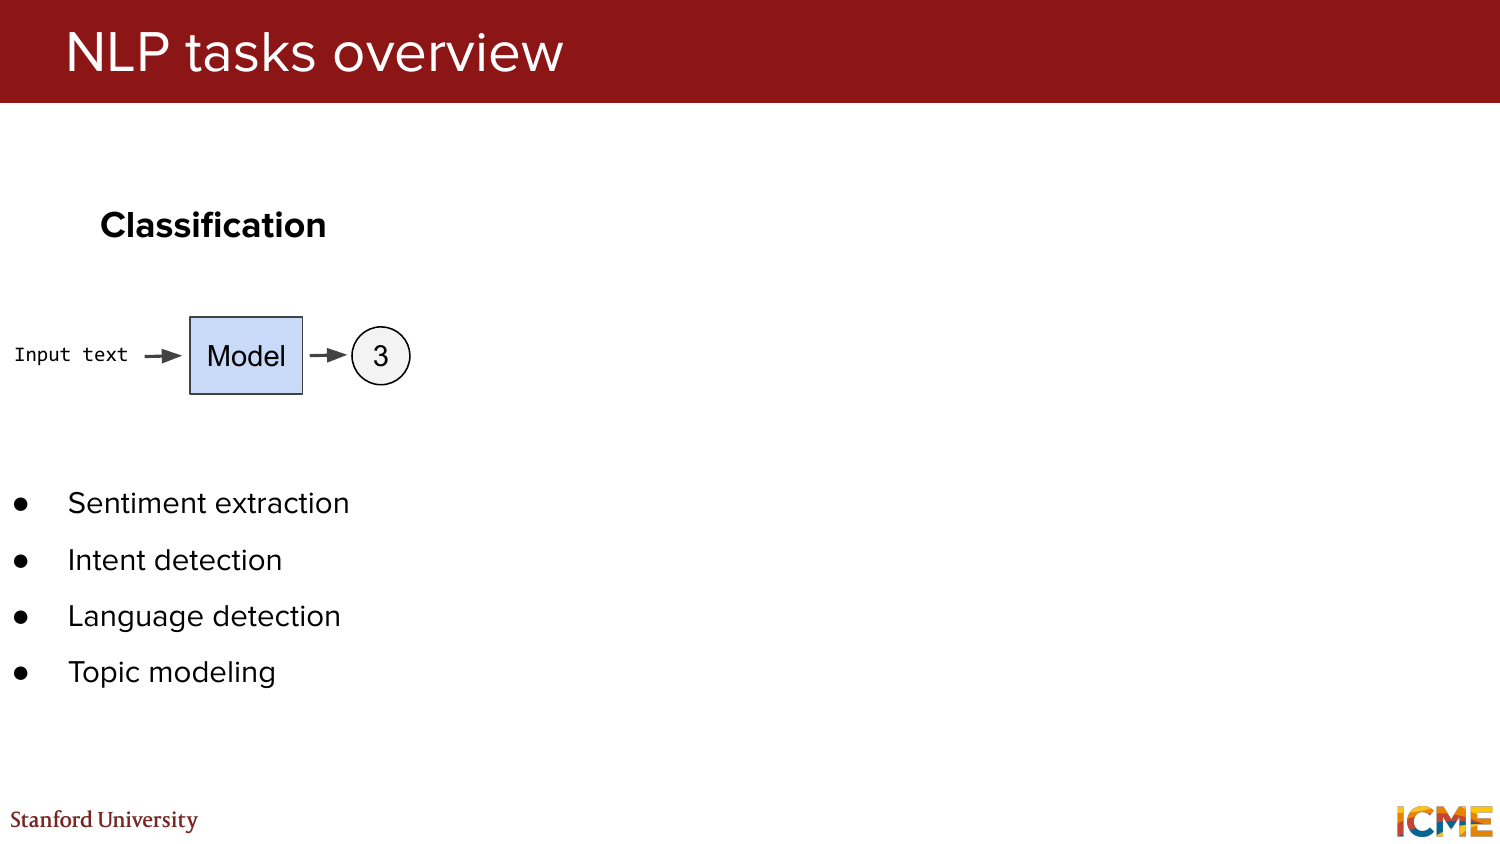
\includegraphics[width=0.92\textwidth]{pdf_pages/page-17.png}
\caption{课程开篇用一张总览图把 NLP 任务分成分类、信息抽取、翻译等大类。}
\end{figure}

课件随后用情感分类、命名实体识别、机器翻译等任务说明 NLP 的输入输出形态并不相同：
\begin{itemize}
\item 分类任务是“文本进，标签出”，例如判断一句话的情感极性。
\item 序列标注任务是“文本进，逐 token 标签出”，例如识别人名、地名、机构名。
\item 生成任务是“文本进，文本出”，例如翻译、摘要、对话生成。
\end{itemize}

这一步并不是背景铺垫而已。它直接服务于后文的架构比较：有些模型适合拿整句表示做预测，有些模型擅长逐 token 条件生成，而 Transformer 之所以重要，是因为它后来演化出了同时覆盖这些任务形态的多种分支。

\begin{importantbox}{时间线的真正含义}
课程中的时间线不是简单罗列年份，而是在说明 NLP 模型设计的焦点如何迁移：先从“如何按顺序处理文本”，发展到“如何学习更有语义的词向量”，再到“如何让任意位置的 token 直接交互”。
\end{importantbox}

\subsection{本章小结}

第一部分的任务是建立全景视角：NLP 并不是一个单一任务，而是一组输入输出模式不同的问题；Transformer 也不是凭空出现，而是为了解决早期方法在表达能力、上下文建模和并行效率上的缺陷。

\section{从分词到词向量：离散文本如何进入神经网络}

模型不能直接处理原始字符串，因此第一步永远是 tokenization。讲者用 ``A cute teddy bear is reading.'' 这个例子说明，分词策略其实对应着不同的工程取舍。

\subsection{分词的三种基本粒度}

课程把分词方法分成三类：
\begin{itemize}
\item 词级分词：直观、可解释，但容易遇到 OOV（out-of-vocabulary）问题，也很难共享词根信息。
\item 子词分词：把高频词保留为整体，把低频词切成可复用片段，在词表规模与泛化能力之间折中。
\item 字符级分词：几乎没有 OOV，但序列会显著变长，模型计算成本变高。
\end{itemize}

\begin{figure}[H]
\centering
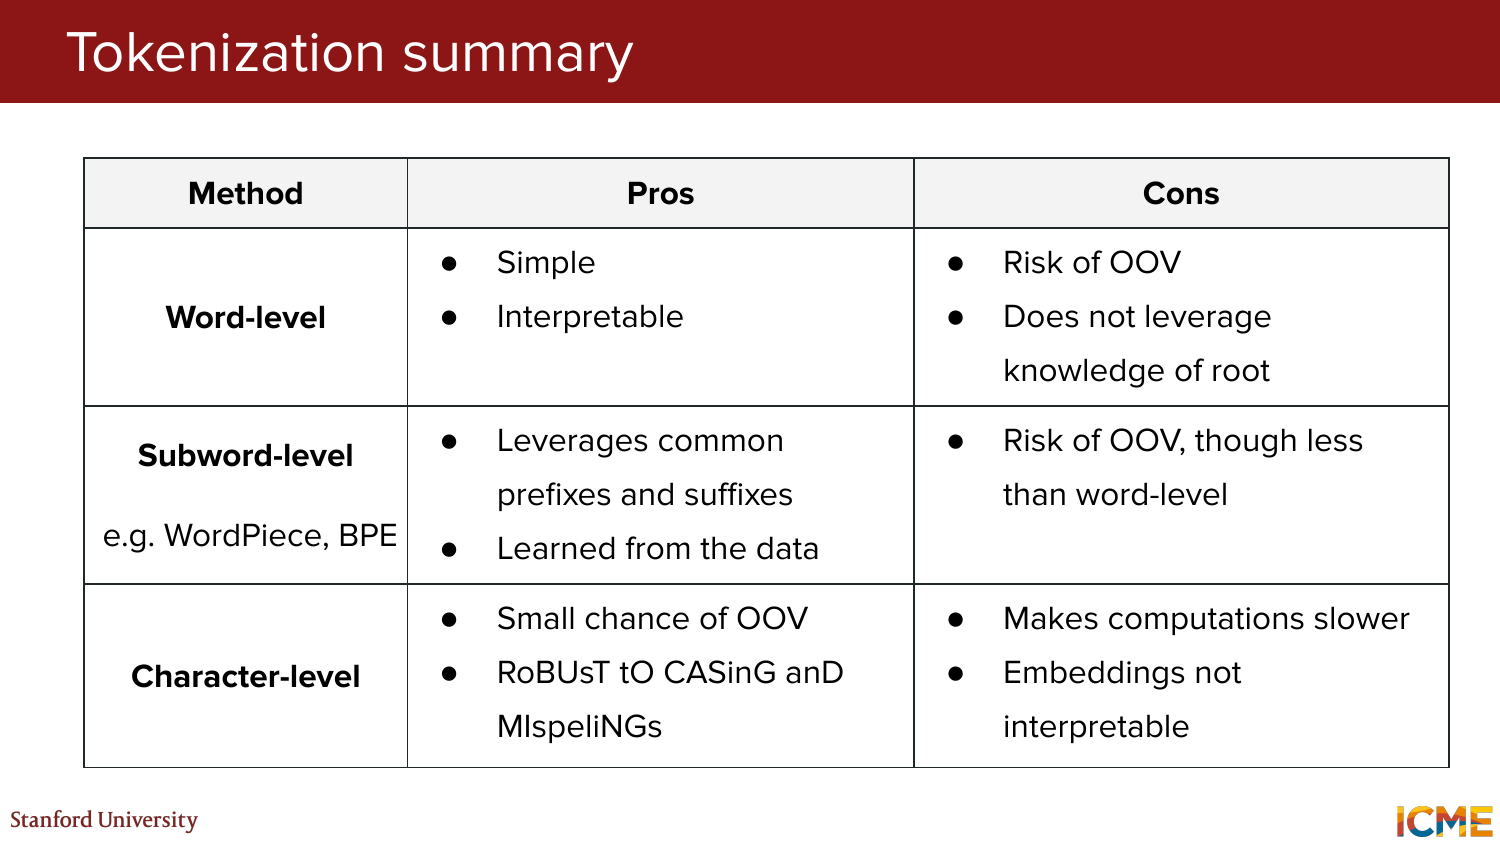
\includegraphics[width=0.95\textwidth]{pdf_pages/page-33.png}
\caption{课件用表格对比词级、子词级、字符级分词的优缺点。}
\end{figure}

讲者特别强调子词分词在现代模型中的关键性。因为语言里既存在常见完整词，也存在大量未登录词、专有名词、拼写变体。子词方法通过复用词根、前后缀和常见片段，让模型既能控制词表规模，又能在新词出现时拼装出可用表示。换句话说，分词并不只是预处理步骤，它直接决定了：
\begin{itemize}
\item 序列长度；
\item 词表大小；
\item OOV 风险；
\item 训练和推理成本。
\end{itemize}

\subsection{从 one-hot 到语义向量}

如果把每个 token 表示成 one-hot 向量，那么不同 token 之间彼此正交，相似词不会更接近，模型也无法从几何结构里复用语义。因此课程引出 token representation，也就是 embedding。

embedding 的目标是把“相似 token 的向量相近、不相似 token 的向量较远”编码进连续空间。这样模型就能用线性层、相似度、聚类等方式直接利用语义结构。

\begin{figure}[H]
\centering
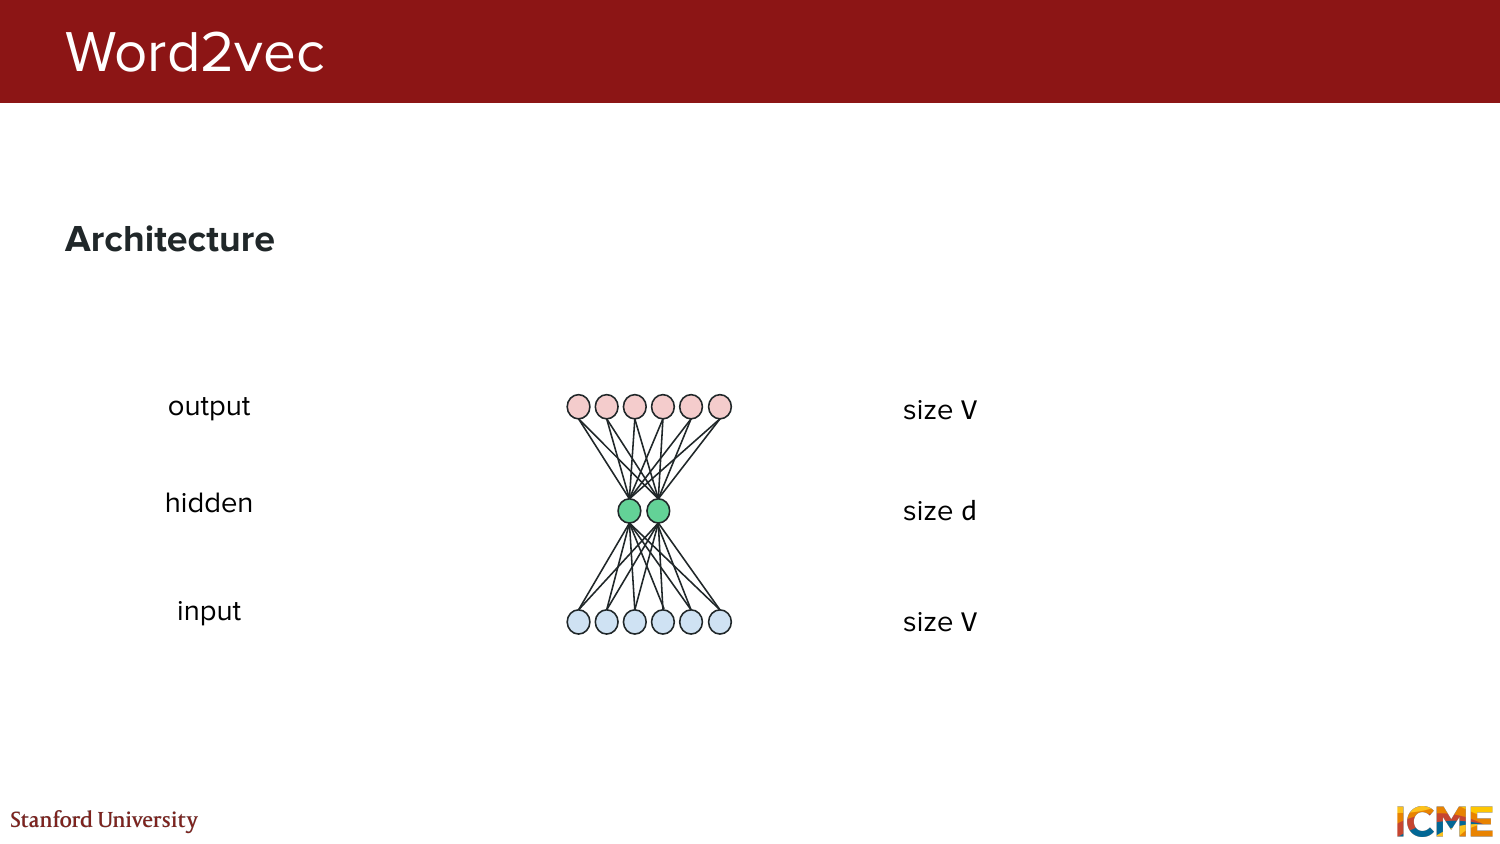
\includegraphics[width=0.78\textwidth]{pdf_pages/page-38.png}
\caption{Word2vec 的基本结构：通过预测上下文或中心词来学习低维词向量。}
\end{figure}

以 Word2vec 为代表的早期词向量方法，其核心思想是“用上下文定义语义”。如果一个词经常出现在相似上下文中，它就应该得到相似表示。课程在这里并不深挖训练细节，而是强调了一个更重要的认识：embedding 不是人工定义的特征，而是通过训练目标从数据中学出来的表示空间。

\begin{warningbox}{静态词向量的局限}
Word2vec 这类方法给同一个 token 分配固定向量，因此无法区分多义词在不同上下文中的含义。后续 RNN、注意力和 Transformer 的发展，本质上都在追求“上下文化表示”。
\end{warningbox}

\subsection{本章小结}

文本进入模型之前必须经历两个步骤：先把字符串切成 token，再把 token 映射成向量。分词控制序列与词表的边界，embedding 则负责把离散符号变成可学习的几何对象。这为后面所有上下文建模方法奠定了输入表示基础。

\section{Transformer 之前：RNN、LSTM 与注意力的动机}

在 Transformer 之前，主流思路是按顺序读入 token。课程用 RNN 和 LSTM 回顾了这种范式的优势与瓶颈。

\subsection{RNN：顺序处理带来的上下文感知}

RNN 的优点在于它按时间顺序处理 token，因此天然保留位置信息。当前时刻的隐藏状态由“当前输入 + 上一时刻状态”共同决定，所以 token 的表示会受前文影响，而不再是静态向量。

\begin{figure}[H]
\centering
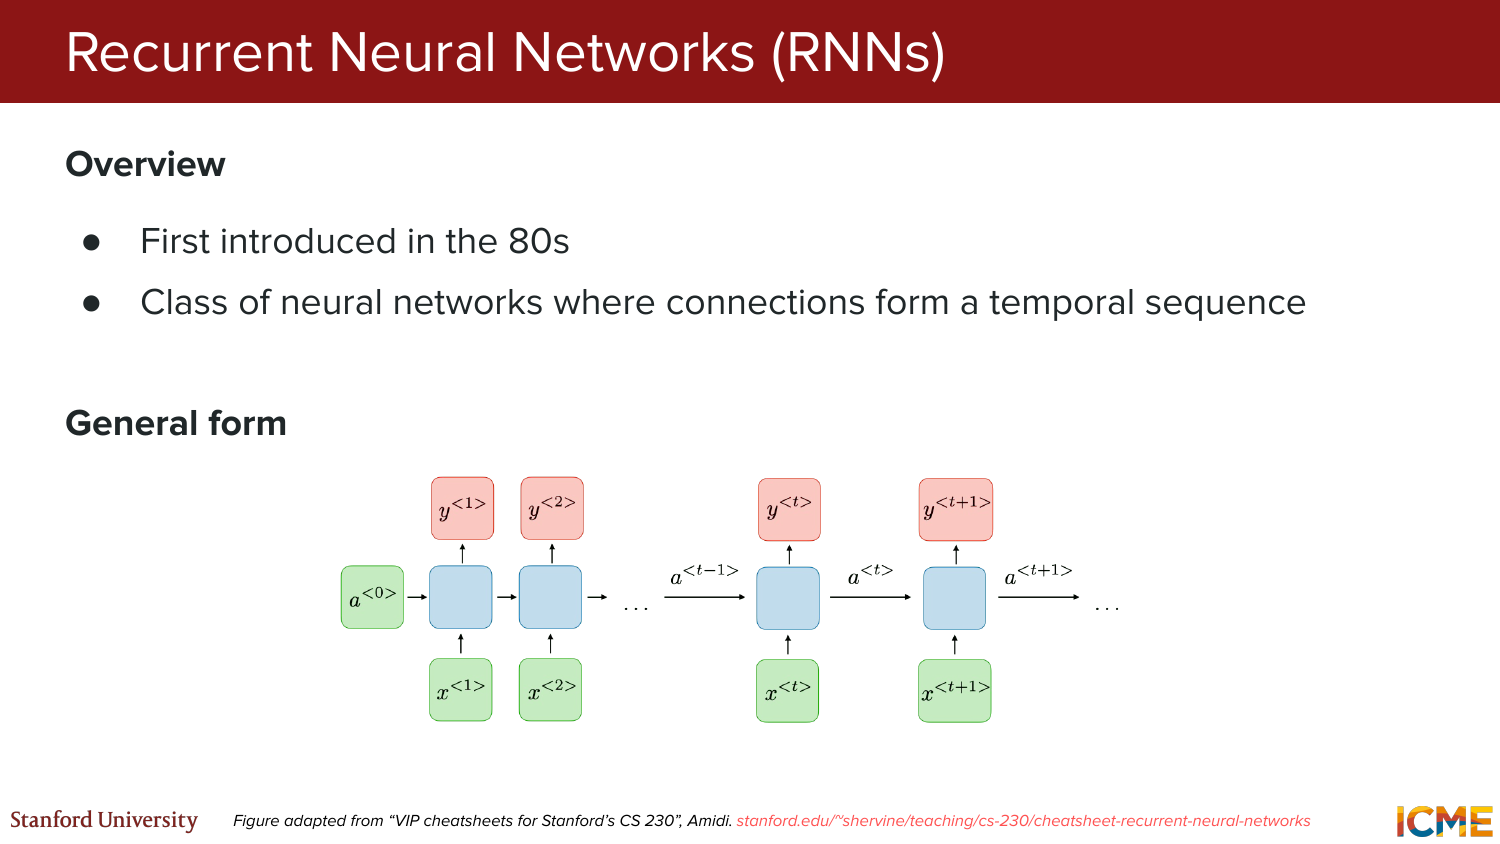
\includegraphics[width=0.88\textwidth]{pdf_pages/page-51.png}
\caption{RNN 通过递归隐藏状态顺序消费 token，从而让词序进入表示。}
\end{figure}

这一步解决了词袋模型和静态 embedding 的一个核心缺陷：词序终于进入模型了。可与此同时，新的问题出现了：
\begin{itemize}
\item 序列必须逐步处理，难以并行；
\item 长程依赖会随着传播路径变长而变得难学；
\item 早期 token 的信息容易在长序列中被冲淡。
\end{itemize}

\subsection{LSTM：对长期依赖的工程修补}

LSTM 通过更复杂的门控结构，让模型在“保留什么、遗忘什么、输出什么”上有了更强控制能力。课程没有把重点放在门控方程推导，而是强调它在历史位置上的作用：LSTM 是对 RNN 长期依赖问题的结构性补救。

\begin{figure}[H]
\centering
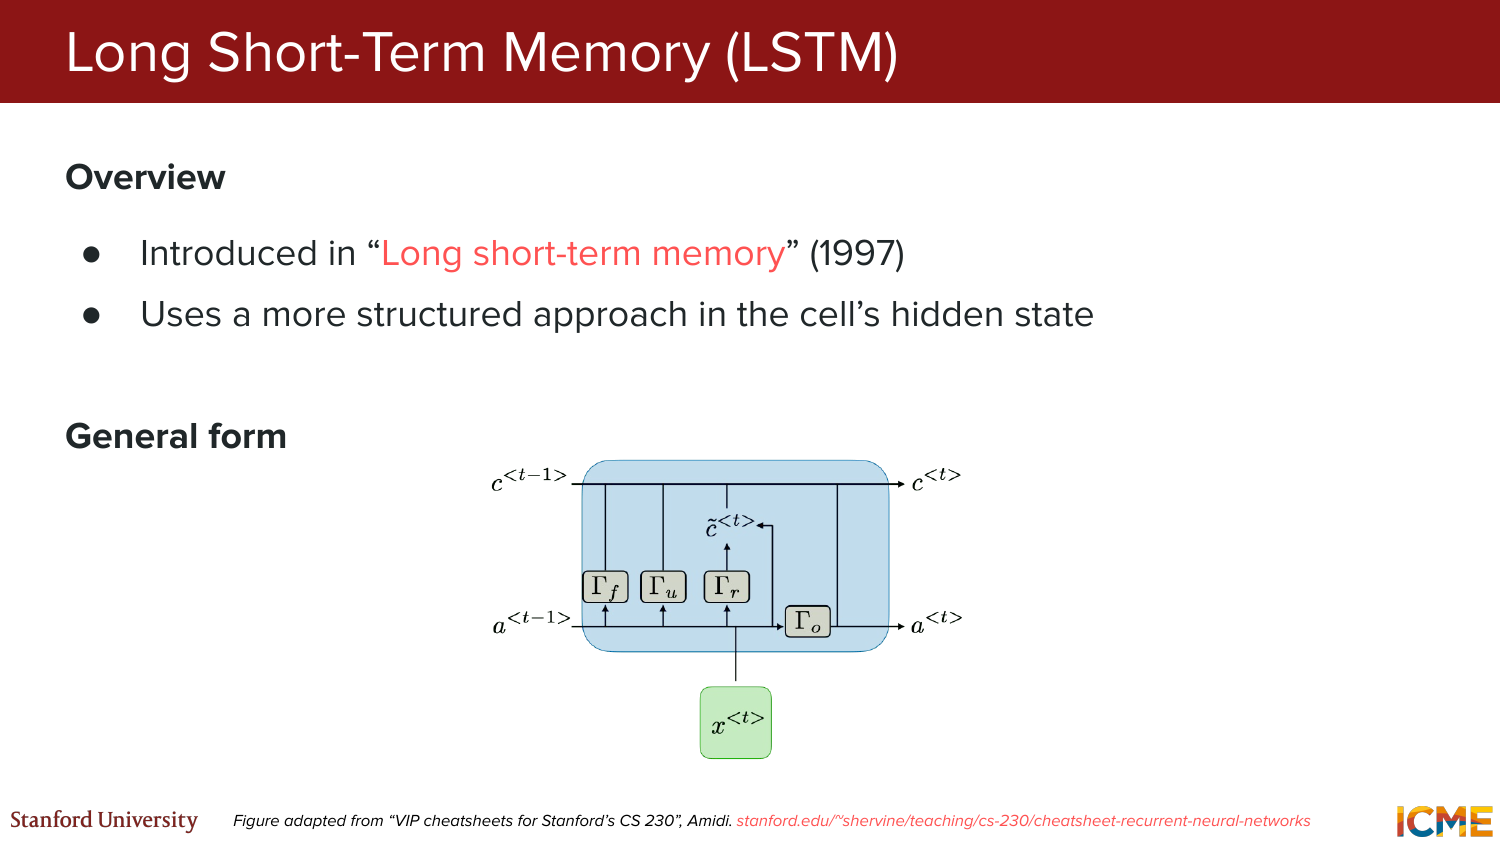
\includegraphics[width=0.78\textwidth]{pdf_pages/page-63.png}
\caption{LSTM 通过更结构化的内部状态和门控机制缓解长期依赖问题。}
\end{figure}

即便如此，LSTM 仍然保留了串行处理的本质。只要模型必须按 token 一个个向前推进，训练和推理就很难充分利用现代硬件的并行矩阵计算能力。

\subsection{注意力为何成为转折点}

课程随后引出 attention 的历史动机：在很多任务中，当前 token 并不只依赖最近一步，而是可能依赖很远位置的若干 token。与其把所有信息强行压缩进一个固定长度状态，不如直接让当前 token “看向”整段上下文中最相关的位置。

这个视角非常关键。它意味着模型不再只能沿着时间链路传递信息，而是可以显式建立“我与谁更相关”的连接。Transformer 正是把这个想法推进到极致。

\subsection{本章小结}

RNN 与 LSTM 的历史作用在于：它们第一次让 token 表示真正依赖上下文，但代价是串行、难并行、长依赖难训练。注意力机制的出现，则把“记住全部过去”改写成“直接访问相关过去”，这就是 Transformer 的前奏。

\section{自注意力机制：让所有 token 直接相互作用}

讲者把自注意力描述为本讲的核心思想。对于一个 token，我们不再只看前一个隐藏状态，而是让它直接与序列中所有 token 交互，并根据相似度聚合信息。

\subsection{Query、Key、Value 的角色分工}

课程用一个直觉化解释来讲 Q、K、V：
\begin{itemize}
\item Query 表示“我正在寻找什么信息”。
\item Key 表示“我这里有什么可供匹配的信息”。
\item Value 表示“一旦我被选中，我实际贡献什么内容”。
\end{itemize}

对某个 token 而言，它会把自己的 query 与所有 token 的 key 做比较，得到相关性权重，再对对应的 value 做加权求和，于是形成一个新的、上下文化的表示。

\begin{figure}[H]
\centering
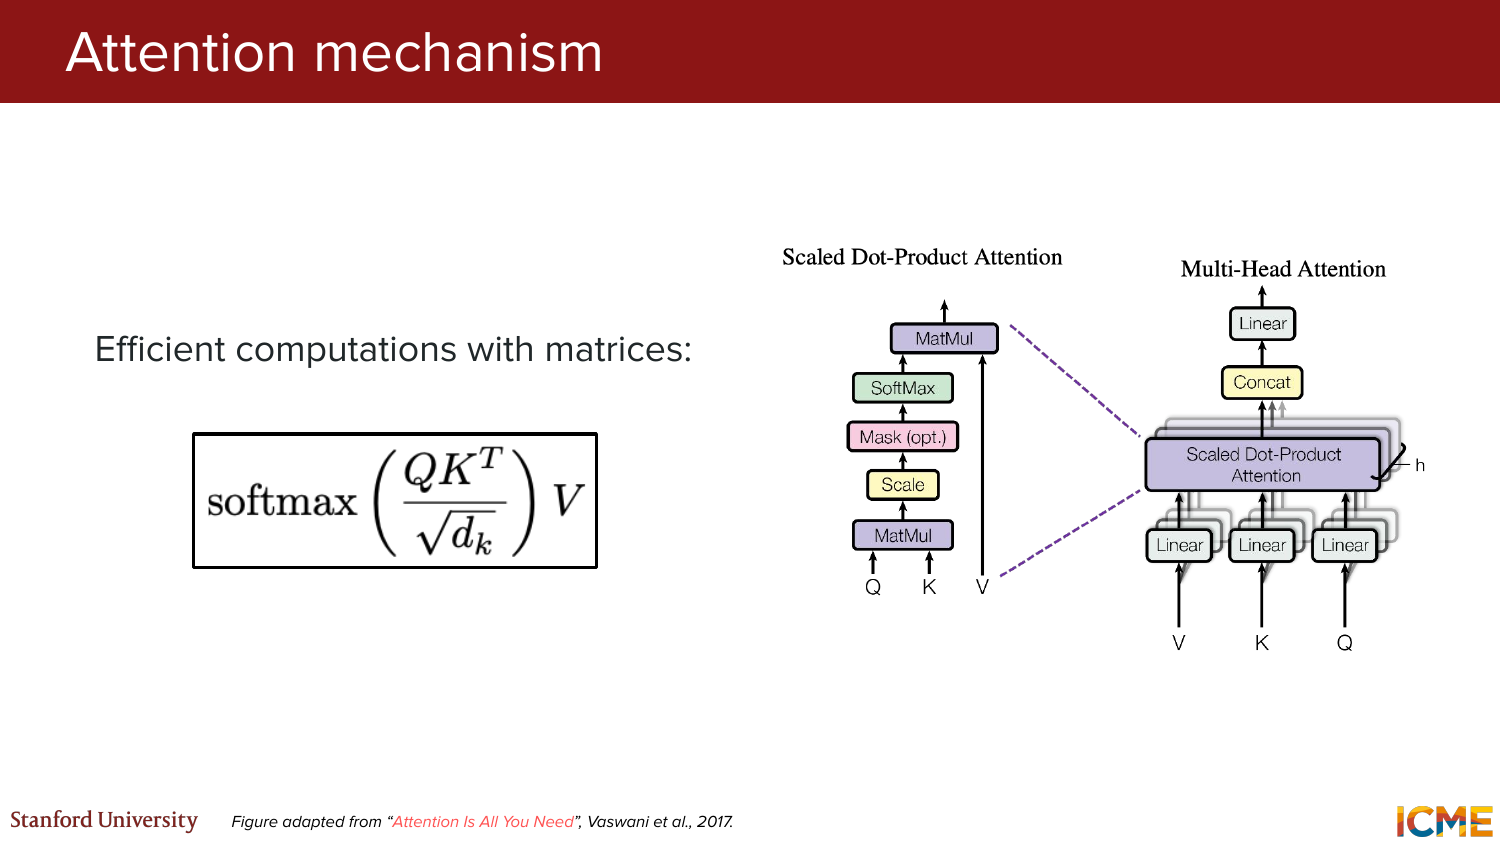
\includegraphics[width=0.88\textwidth]{pdf_pages/page-78.png}
\caption{自注意力把相似度计算写成统一的矩阵形式，从而适合硬件并行。}
\end{figure}

\subsection{注意力公式与含义}

课程给出的标准形式是：
\[
\mathrm{Attention}(Q, K, V)=\mathrm{softmax}\left(\frac{QK^\top}{\sqrt{d_k}}\right)V
\]

式中各符号的含义如下：
\begin{itemize}
\item \(Q\)：所有 query 组成的矩阵；
\item \(K\)：所有 key 组成的矩阵；
\item \(V\)：所有 value 组成的矩阵；
\item \(QK^\top\)：两两 token 的相关性分数；
\item \(d_k\)：key 的维度，用 \(\sqrt{d_k}\) 缩放是为了稳定数值范围；
\item \(\mathrm{softmax}\)：把分数变成权重分布；
\item 最终结果：对 value 的加权和，即新的上下文化表示。
\end{itemize}

这个公式最重要的不是记忆，而是理解它为什么高效。过去 RNN 风格方法依赖时间步递推；这里则把大量关系计算写成矩阵乘法和 softmax，因此可以在硬件上高度并行。

\begin{knowledgebox}{为什么说自注意力是“上下文化 embedding”？}
因为输出不再只是 token 自己的静态表示，而是融合了整段序列中与它最相关的信息。一个 token 的新向量，取决于同一句话中其他 token 对它的贡献。
\end{knowledgebox}

\subsection{多头注意力的意义}

课程最后补充了 multi-head attention 的直觉：不要只学习一种相似性，而是并行学习多种投影空间。不同 head 可能分别关注语法关系、指代关系、局部搭配或长程语义线索。训练过程中虽然没有硬性约束要求各 head 分工不同，但梯度下降往往会驱动它们学出互补表示。

\subsection{本章小结}

自注意力把序列建模从“按时间递推”改成“按相关性聚合”。Q/K/V 提供了统一接口，矩阵形式提供了并行能力，多头机制则让模型能够在多个关系子空间里同时建模。这是 Transformer 优于早期序列模型的第一根支柱。

\section{Transformer 架构：从输入到翻译输出的完整数据流}

当自注意力被组织进 encoder-decoder 框架时，Transformer 便成形了。课程这一部分最重要的价值在于：它不是只给出模块名称，而是用一个翻译示例把信息流串了起来。

\begin{figure}[H]
\centering
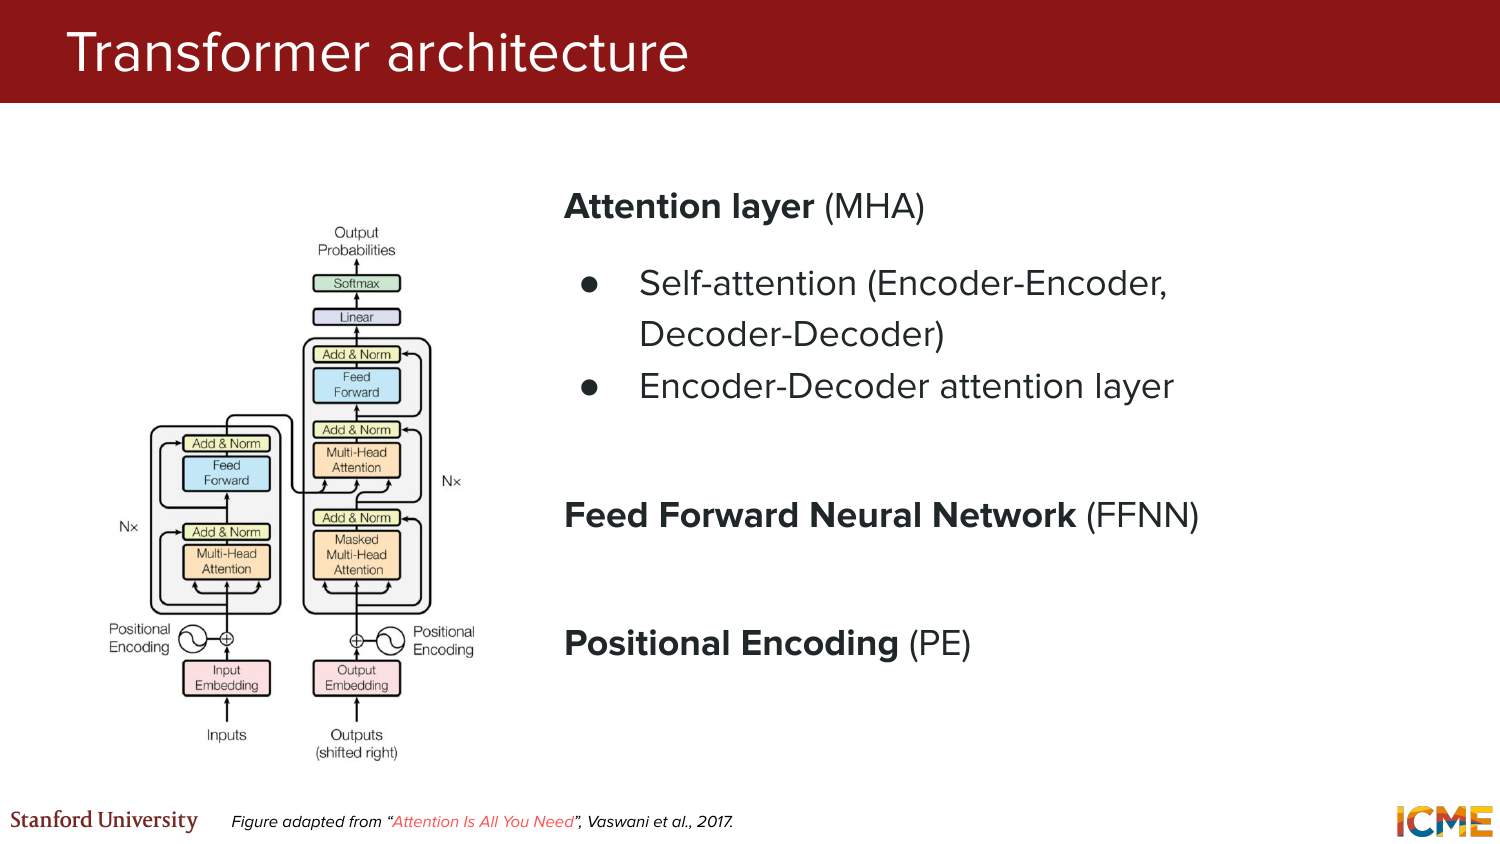
\includegraphics[width=0.78\textwidth]{pdf_pages/page-80.png}
\caption{Transformer 的总架构：编码器负责输入表征，解码器负责条件生成。}
\end{figure}

\subsection{输入侧：token embedding 加位置编码}

由于自注意力本身不保留顺序，输入 token embedding 必须补上 positional encoding。课程在这一讲只给概念，不展开具体构造方法，但已经给出清晰定位：位置编码不是额外点缀，而是让模型分辨顺序的必要信号。

编码器侧的数据流可以概括为：
\begin{enumerate}
\item 文本被切成 token；
\item token 被映射成 embedding；
\item 加入位置编码形成 position-aware embeddings；
\item 送入多层 encoder block。
\end{enumerate}

\subsection{编码器与解码器各做什么}

每个 encoder block 主要包含两类子层：
\begin{itemize}
\item 多头自注意力层：让输入序列内部充分交互；
\item 前馈网络（FFN）：对每个位置的表示做更强的非线性变换。
\end{itemize}

解码器则更复杂一些，它既要看已经生成的输出前缀，又要看编码器产出的输入表示，因此包含：
\begin{itemize}
\item masked self-attention：只能看当前位置左侧，保证因果性；
\item cross-attention：把解码器当前状态与编码器输出对齐；
\item FFN：进一步丰富表示。
\end{itemize}

\subsection{为什么需要 masked self-attention 与 cross-attention}

masked self-attention 的目的是防止信息泄漏。做下一个 token 预测时，模型不能偷看未来 token，因此解码器每个位置只能访问自己和之前位置。

cross-attention 则承担“条件生成”的角色。解码器当前状态提出 query，编码器输出提供 key 和 value，模型据此决定源句中哪些位置最有助于当前目标词生成。机器翻译正是这种结构最典型的应用：左边编码英文句子，右边逐词解码法文句子。

\begin{figure}[H]
\centering
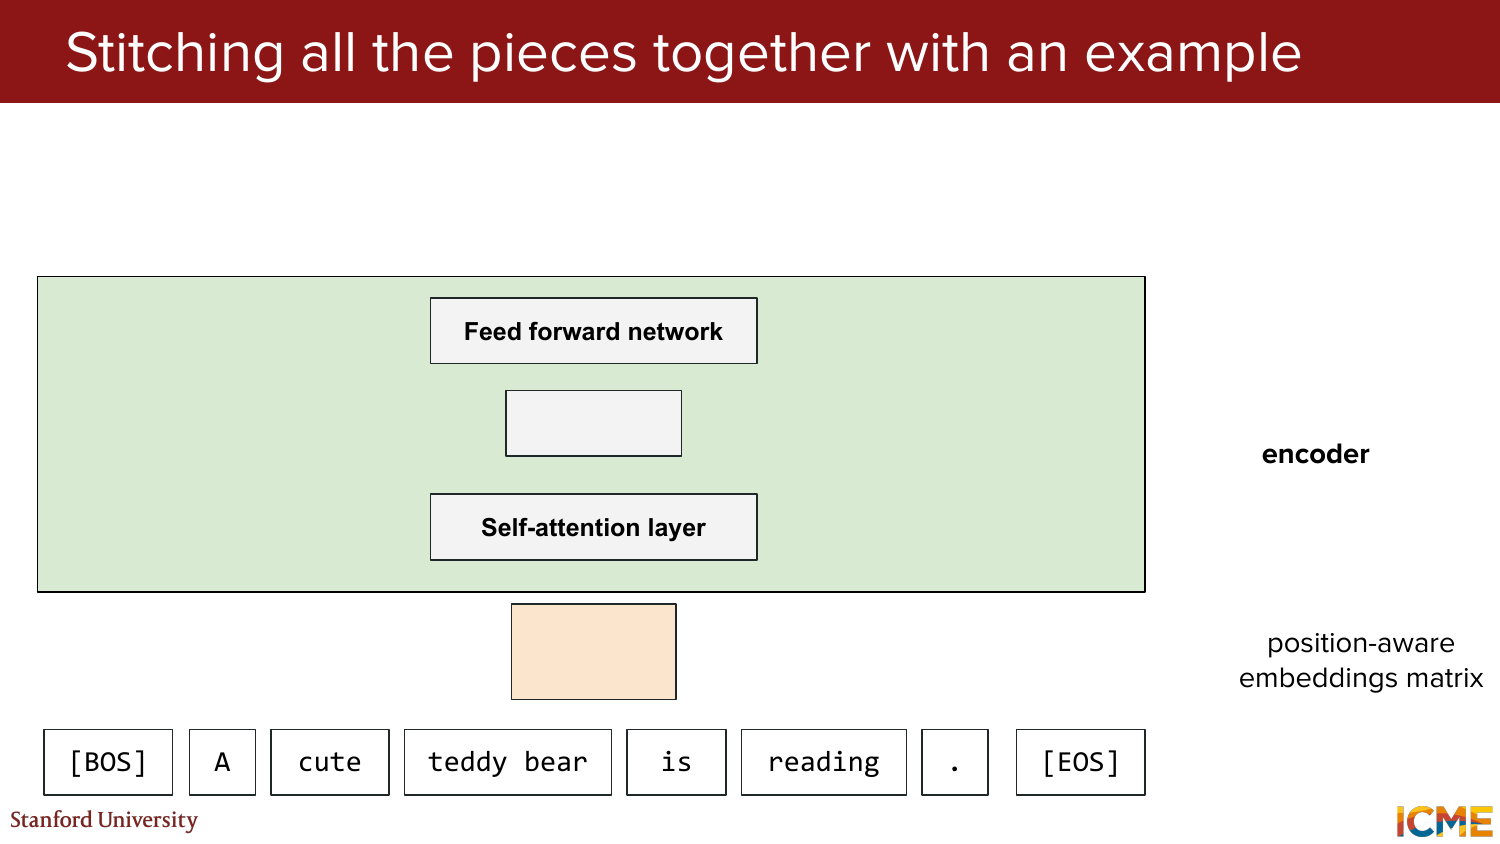
\includegraphics[width=0.92\textwidth]{pdf_pages/page-115.png}
\caption{课件通过逐步拼装示例，把 embedding、自注意力、FFN 和 encoder 串成一条可追踪的数据流。}
\end{figure}

\subsection{计算技巧与训练细节}

课程还点到两个原始 Transformer 论文中的重要技巧：
\begin{itemize}
\item Multi-head attention：让多组投影并行工作，增强表达能力；
\item Label smoothing：在训练时避免目标分布过于尖锐，改善泛化和校准。
\end{itemize}

另外，FFN 的隐藏层通常比输入输出维度更大。讲者在问答里明确说明，这样做是为了给模型更高的特征变换自由度，而不是像 Word2vec 那样做压缩瓶颈。

\subsection{生成过程的闭环}

解码从 \texttt{[BOS]} 开始，模型在 softmax 层上得到整个词表的概率分布，选出下一个 token 后再送回解码器继续迭代。当生成到 \texttt{[EOS]} 时，序列结束。这个循环就是后续所有自回归语言模型推理的基础范式。

\subsection{本章小结}

Transformer 可以看成把“位置编码 + 自注意力 + FFN + 因果掩码 + 编解码交互”系统性拼接在一起。编码器负责把输入压成上下文化表示，解码器负责在条件约束下逐 token 生成输出，而这套流程后来成为现代大语言模型演化的出发点。

\section{总结与延伸}

这节课的真正任务不是把 Transformer 一次性讲到最细，而是搭建一条完整的认知路径：
\begin{enumerate}
\item 文本必须先被切成 token，并映射为向量；
\item 静态 embedding 不够，因为语义依赖上下文；
\item RNN/LSTM 虽然能建模顺序，但串行且难处理长程依赖；
\item 注意力机制允许 token 直接访问相关上下文；
\item Transformer 把注意力机制工程化、模块化，并借助矩阵并行获得巨大可扩展性。
\end{enumerate}

如果把本讲看成整门课的地基，那么最值得带走的不是若干缩写，而是三条主线：
\begin{itemize}
\item \textbf{表示主线}：从离散 token 到上下文化向量表示；
\item \textbf{结构主线}：从顺序递推到全局交互；
\item \textbf{计算主线}：从难并行的时间链路到适合硬件的矩阵运算。
\end{itemize}

后续课程将在这个基础上继续展开：第二讲会讨论位置编码、归一化和模型变体，第三讲则会真正进入大语言模型本体，包括解码策略、提示学习和推理优化。回看本讲，Transformer 之所以成为主角，并不是因为名字响亮，而是因为它第一次把“表达能力”“全局依赖建模”和“可扩展计算”同时放进了同一套架构里。

\end{document}
